\documentclass[journal]{vgtc}                % final (journal style)
%\documentclass[review,journal]{vgtc}         % review (journal style)
%\documentclass[widereview]{vgtc}             % wide-spaced review
%\documentclass[preprint,journal]{vgtc}       % preprint (journal style)

%% Uncomment one of the lines above depending on where your paper is
%% in the conference process. ``review'' and ``widereview'' are for review
%% submission, ``preprint'' is for pre-publication, and the final version
%% doesn't use a specific qualifier.

%% Please use one of the ``review'' options in combination with the
%% assigned online id (see below) ONLY if your paper uses a double blind
%% review process. Some conferences, like IEEE Vis and InfoVis, have NOT
%% in the past.

%% Please note that the use of figures other than the optional teaser is not permitted on the first page
%% of the journal version.  Figures should begin on the second page and be
%% in CMYK or Grey scale format, otherwise, colour shifting may occur
%% during the printing process.  Papers submitted with figures other than the optional teaser on the
%% first page will be refused. Also, the teaser figure should only have the
%% width of the abstract as the template enforces it.

%% These few lines make a distinction between latex and pdflatex calls and they
%% bring in essential packages for graphics and font handling.
%% Note that due to the \DeclareGraphicsExtensions{} call it is no longer necessary
%% to provide the the path and extension of a graphics file:
%% 
\includegraphics{diamondrule} is completely sufficient.
%%
\ifpdf%                                % if we use pdflatex
  \pdfoutput=1\relax                   % create PDFs from pdfLaTeX
  \pdfcompresslevel=9                  % PDF Compression
  \pdfoptionpdfminorversion=7          % create PDF 1.7
  \ExecuteOptions{pdftex}
  \usepackage{graphicx}                % allow us to embed graphics files
  \DeclareGraphicsExtensions{.pdf,.png,.jpg,.jpeg} % for pdflatex we expect .pdf, .png, or .jpg files
\else%                                 % else we use pure latex
  \ExecuteOptions{dvips}
  \usepackage{graphicx}                % allow us to embed graphics files
  \DeclareGraphicsExtensions{.eps}     % for pure latex we expect eps files
\fi%

%% it is recomended to use ``\autoref{sec:bla}'' instead of ``Fig.~\ref{sec:bla}''
\graphicspath{{figures/}{pictures/}{images/}{./}} % where to search for the images

\usepackage{microtype}                 % use micro-typography (slightly more compact, better to read)
\PassOptionsToPackage{warn}{textcomp}  % to address font issues with \textrightarrow
\usepackage{textcomp}                  % use better special symbols
\usepackage{mathptmx}                  % use matching math font
\usepackage{times}                     % we use Times as the main font
\renewcommand*\ttdefault{txtt}         % a nicer typewriter font
\usepackage{cite}                      % needed to automatically sort the references
\usepackage{tabu}                      % only used for the table example
\usepackage{booktabs}                  % only used for the table example
%% We encourage the use of mathptmx for consistent usage of times font
%% throughout the proceedings. However, if you encounter conflicts
%% with other math-related packages, you may want to disable it.

%% In preprint mode you may define your own headline.
%\preprinttext{To appear in IEEE Transactions on Visualization and Computer Graphics.}

%% If you are submitting a paper to a conference for review with a double
%% blind reviewing process, please replace the value ``0'' below with your
%% OnlineID. Otherwise, you may safely leave it at ``0''.
\onlineid{0}

%% declare the category of your paper, only shown in review mode
\vgtccategory{Research}
%% please declare the paper type of your paper to help reviewers, only shown in review mode
%% choices:
%% * algorithm/technique
%% * application/design study
%% * evaluation
%% * system
%% * theory/model
\vgtcpapertype{please specify}

%% Paper title.
\title{Assignment 2 - CS 458}

%% This is how authors are specified in the journal style

%% indicate IEEE Member or Student Member in form indicated below
\author{Amber Horvath, Alannah Oleson, and Katherine Bajno}
\authorfooter{
%% insert punctuation at end of each item
\item
 Amber Horvath, computer science student at Oregon State University: E-mail: horvatha@oregonstate.edu.
\item
 Alannah Oleson, computer science student at Oregon State University. E-mail: olesona@oregonstate.edu.
\item
 Katherine Bajno, computer science student at Oregon State University. E-mail: kbajno@oregonstate.edu
}

%other entries to be set up for journal
%\shortauthortitle{Firstauthor \MakeLowercase{\textit{et al.}}: Paper Title}

%% Abstract section.
\abstract {
On a large scale, many recent studies link high air pollution levels to the larger problem of climate
change. On a somewhat smaller scale, a large amount of air pollution can not only affect the climate
of a certain geographic region - it can also negatively affect the quality of life for those who
live there. Over time, the rate at which the air quality of a region is increasing or decreasing
can single the area out for inspection by climate scientists or give the inhabitants of the area
an indicator of the overall healthiness of the environment there.

To address both issues in a way that the average person can understand, we created a 
visualization of air pollution levels in the western United States. We use a treemap format
to represent the magnitude of 11 states' air pollution levels over the span of ten years. 
We also make use of a color gradient to indicate the rate at which polltion levels are increasing
or decreasing. This is a novel representation because much of this kind of data is presented in 
tables that are rather hard to parse. Our visualization, on the other hand, gives the user a good 
overview of general trends in the region at a glance, while still allowing them to drill down into
the details if they want to. This can benefit both average people (for instance, someone looking at
which state in the region they want to move to) and those with specialized needs such as climate
scientists.
}
% end of abstract

%% Keywords that describe your work. Will show as 'Index Terms' in journal
%% please capitalize first letter and insert punctuation after last keyword
%\keywords{Radiosity, global illumination, constant time}

%% ACM Computing Classification System (CCS). 
%% See <http://www.acm.org/class/1998/> for details.
%% The ``\CCScat'' command takes four arguments.



%% Uncomment below to include a teaser figure.


%% Uncomment below to disable the manuscript note
\renewcommand{\manuscriptnotetxt}{}

%% Copyright space is enabled by default as required by guidelines.
%% It is disabled by the 'review' option or via the following command:
% \nocopyrightspace

\vgtcinsertpkg

%%%%%%%%%%%%%%%%%%%%%%%%%%%%%%%%%%%%%%%%%%%%%%%%%%%%%%%%%%%%%%%%
%%%%%%%%%%%%%%%%%%%%%% START OF THE PAPER %%%%%%%%%%%%%%%%%%%%%%
%%%%%%%%%%%%%%%%%%%%%%%%%%%%%%%%%%%%%%%%%%%%%%%%%%%%%%%%%%%%%%%%%

\begin{document}

%% The ``\maketitle'' command must be the first command after the
%% ``\begin{document}'' command. It prepares and prints the title block.

%% the only exception to this rule is the \firstsection command
%\firstsection{Introduction}

\maketitle

\section{Introduction} %for journal use above \firstsection{..} instead

\subsection{Problem}
Within the last decade, numerous works have surfaced that suggest climate change has detrimental effects on many 
aspects of the environment. One indicator of climate change in a geographic region is air quality, which is measured 
in parts per million of particulate matter. Generally, any particulate less than 2.5 microns in diameter meets the 
standards for “dangerous” particulates. An area that has a high concentration of dangerous particulates - a high 
number on the air quality index, which corresponds to bad air quality - can be both a symptom of or a catalyst for 
climate change. Identifying areas in which the air quality is markedly bad or decreasing over time can provide a way 
to focus climate change studies and environmental science efforts.

\subsection{Motivation}
Though there is much data available on the topic of air quality, very little of it is not simply presented in a table 
or list. Of the visualizations that do exist, many are simply colored maps that make darker or more saturated colors 
correspond to worse air qualities. Thus, it can be hard to see just which areas present a problem over time (
signified by either a continual or sudden, severe decrease in air quality). A visualization that could clearly show 
both the magnitude of the air quality index and give an indication of how the quality was increasing or decreasing 
over time would be very useful to researchers in the field and those who want to see a simple version of the data
to quickly grasp the concepts.

\subsection{Potential Users}
Our potential users include researchers and climate change/air quality scientists who study geographic regions in the 
western US. (We will focus our visualization on this region in order to make the scope appropriate for this project.) 
This visualization will ideally give scientists a quick overview of air quality trends in an area, which could 
indicate that the region requires more study or analysis in future work.

In addition, we should not forget that the general population might benefit from a good visualization of this data as 
well. For instance, perhaps a person who has asthma might view the data as part of a decision on whether or not to 
relocate to a certain state. A citizen activist might also be interested in this data in order to raise awareness in 
their region about the dangers of poor air quality. Multiple cases such as these exist and might be well served by 
this visualization. We will focus on this demographic when developing our visualization.

\subsection{General Approach}
We will pull data from the American Health Rankings site by the United Health Foundation. We will use this to 
aggregate data from the air quality measures of 13 western region states over the past 10 years. We then intend to 
make a 
series of tree maps that visualize two dimensions of the data: the magnitude of the air pollution levels (represented 
by the size of the block; larger = worse) and the rate of change in air quality levels (represented by the color of 
the block; blue = decreasing/getting better, orange = increasing/getting worse, more saturated = changing faster).

\section{Visualization Tasks}

\begin{itemize}
\item Our visualization aims to address the following questions:
  \begin{itemize}
    \item How fast is the air quality increasing and decreasing in each state?
    \item What states on the west coast are most at risk of bad air quality?
    \item What trends in air quality can we identify in air quality on the west coast over the past 10 years?
    \item Which states can be identified as “danger zones” for further research (air pollution that is quickly increasing)?
  \end{itemize}
\end{itemize}


\section{Related Work}

Climate change has been studied by many research groups across different domains. However, how groups choose to visualize
the data changes depending upon the focus of the group and what questions they're trying to answer. The team's software
capabilities also come in to play, with some groups researching air pollution having little to no background in 
programming or information visualization. Zell et al. (2010) found that, between the years 1955 and 2006, 
26,253 different titles were published relating to air pollution from 124 different countries [Zell et al. 2010]. 


Judging by this influx of publications, air pollution is clearly an issue that has garned interest from people of all
backgrounds and interests. It is also important to note that humans play a large role in air pollution, with
NASA releasing satellite visualizations of our impact on air quality [NASA]. Air pollution is also extremely dangerous,
with an estimated 2.4 million fatalities occurring each year due to unsafe living conditions caused by air pollution [WHO].
Different groups of researchers have attempted to create visualizations that both inform
experts and the general public while also being used to glean meaningful information about different atmospheric trends.

In an effort to inform city planners on how to structure future traffice schemes, Zahran et al. ran a case study
to test their implementation of a 3D city model with an overlay of the changing air pollution through different types of
visualizations[Zahran et al.]. 
Through their different tests, they found that users best understood the metaphor of smog clouds 
covering the more polluted areas and less clouds over the more clear areas.
Perhaps an easily understandable metaphor is a good way to inform the public on levels of air pollution - however, how
to do this on a state by state basis and capture the temporal aspect may not be possible with the cloud metaphor. 

Elbir created a system to estimate the ambient air pollution levels temporally and spatially with the goal of mapping
emissions and air quality levels [Elbir 2004]. 
The target users are policy makers in order to inform and predict air quality changes within the region they are 
evaluating. Elbir uses darker markings on a map of the area to show concentration of harmful air pollutants.
The advantage of Elbir's system is that, not only does it visualize current air pollution, it also predicts future
pollution levels based upon the data currently available. This might be an avenue of future research for our
visualization to help citizens of the states we are visualizing to better understand whether their state is at risk or
to see if it is imporiving over time. 

Wang et al. created a viewpoint-based method for rendering of visualizations that promotes speed and interactivity [Wang 
et al 2010]. Speed is important as, if the data is consistently being sampled, being able to render and update on the 
fly leads to the most accurate and relevant information being shared. This type of sampling is important for government
officials to keep their patrons informed if a certain area is reaching dangerous levels of pollution. The scope of our
project does not reach that level of criticality, but if we shifted our audience towards government officials, their
system might be an avenue for implementation efforts.

The kind of work Wang et al. are doing is similar to the work of Li et al. Li et al. aimed to create many different
visualizations to inform policy makers in Beijing what is causing the rapid increase in air pollution and to analyze
the trends in order to combat the air pollution [Li et al 2016]. The authors attempted different methods of 
visualizations and found certain types of visualizations lead to different information being conveyed (e.g. scatter
plots helped locate where data was missing). The authors also found that wind speed affected change in air pollution.
Li et al. also leveraged some open source software in order to create their visualization. One such open source software is
Openair, an R software package used to visual air quality [Openair].
These findings suggest our visualization could be improved through supporting different visualizations depending
upon what question the user is trying to answer through our visualization. For future work, we might also consider
leveraging some of these open source software options in order to keep our product flexible and receptive to incoming
data.

Another different type of visualization researchers have tried is Bi et al.'s tree visualization [Bi et al.]. The tree is
used to represent different polutant levels for each day throughout a month in a given area. This metaphor allows for
a high level of accuracy, but does not provide a broader scale view or allow for easy comparison between different regions.

Beyond purely visualizations but in the vein of informing the public, 
Bohler et al. developed a system called APNEE (Air Pollution Network for Early warning and online information Exchange in
 Europe) as a ways of informing select citizens through mobile messages, online posts, and street panels when air pollution
 reaches certain critical levels [Bohler et al.]. 
 Perhaps if we leveraged our software beyond merely a visualization and created an app, we
 could also distribute our information to patrons. For now, that is outside of the scope of our assignment, and wouldn't
 make a lot of sense unless we had more frequent updates on climate change (currently our system functions on a year-long
 comparison level).



\section{Background}
After doing a review of previous literature, we found most previous reseach was aimed at informing policy makers
and other officials of the state of their local air pollution rates. These visualizations, while similar to our work,
differ slightly in that they are made by experts for experts. In our case, we are seeking to inform the greater public
on a more general level of how their state is doing in comparison to other states and whether their state's air pollution
is increasing or decreasing. Our goal is to provide an easy to understand visualization for non-experts to track their
state's pollution levels.

\section{Methods}
\subsection{Data Sources}

We will be pulling data from the United Health Foundation’s website that catalogues data about each state by year. We 
will be studying 11 different states in the western US. We chose the western United States as the data set was 
relevant to our team's interest and to keep the project within a manageable scope. In addition, since we all live in the
western US, this topic was of particular interest to our team: many of us intend to live and work in the Pacific 
Northwest. Therefore, we can use our visualization to help us determine what states we could end up in.
\begin{itemize}
\item Washington: 
http://www.americashealthrankings.org/explore/2015-annual-report/measure/air/state/WA
\item Oregon: http://www.americashealthrankings.org/explore/2015-annual-report/measure/air/state/OR
\item California: http://www.americashealthrankings.org/explore/2015-annual-report/measure/air/state/CA
\item Alaska: http://www.americashealthrankings.org/explore/2015-annual-report/measure/air/state/AK 
\item Hawaii: http://www.americashealthrankings.org/explore/2015-annual-report/measure/air/state/HI
\item Montana: http://www.americashealthrankings.org/explore/2015-annual-report/measure/air/state/MT
\item Wyoming: http://www.americashealthrankings.org/explore/2015-annual-report/measure/air/state/WY
\item Colorado: http://www.americashealthrankings.org/explore/2015-annual-report/measure/air/state/CO
\item New Mexico: http://www.americashealthrankings.org/explore/2015-annual-report/measure/air/state/NM
\item Idaho: http://www.americashealthrankings.org/explore/2015-annual-report/measure/air/state/ID
\item Utah: http://www.americashealthrankings.org/explore/2015-annual-report/measure/air/state/UT
\item Arizona: http://www.americashealthrankings.org/explore/2015-annual-report/measure/air/state/AZ
\item Nevada: http://www.americashealthrankings.org/explore/2015-annual-report/measure/air/state/NV 
\end{itemize}


\subsection{Data Organization}

We set up our data in the form of 3 tables: 1 for the states, one for the years, and one for the air pollution. The 
entity-relationship diagram for these tables can be seen in Figure \ref{fig:ERdiagram}. 
The state name and year are used as keys to index the values stored within the air pollution table. This data was 
retrieved from the United Health Foundation's report on air pollution across the United States.

This database was hosted on Oregon State University's ONID database service during early testing. For ease of development,
we later moved to to Amazon Web Service databases. This allowed us to better leverage external JavaScript libraries
when developing the interface.

\begin{figure}
 \centering % avoid the use of \begin{center}...\end{center} and use \centering instead (more compact)
 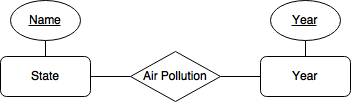
\includegraphics[width=\columnwidth]{cs458-ER-diagram-ass1.png}
 \caption{An ER diagram showing the relationship between our 3 tables: the State table has a primary key "name" and the Year table has a primary key "year", both of which are used to query on the Air Pollution table}
 \label{fig:ERdiagram}
\end{figure}


\begin{figure}
\centering
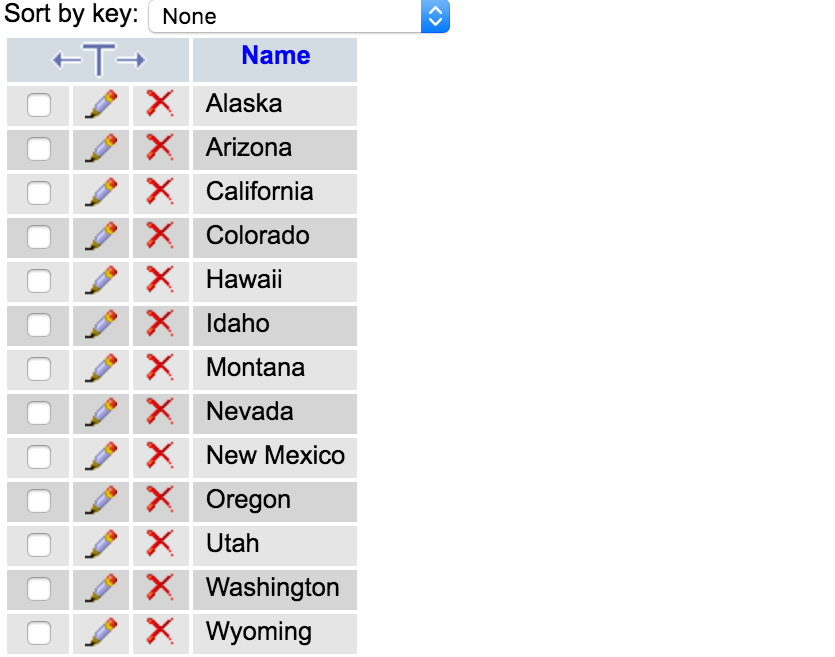
\includegraphics[width=\columnwidth]{state_db.png}
\caption{A visualization of the contents of the "state" table, with the "name" column serving as the primary key and key 
to index the "air pollution" table.}
\label{fig:stateDB}
\end{figure}

\begin{figure}
\centering
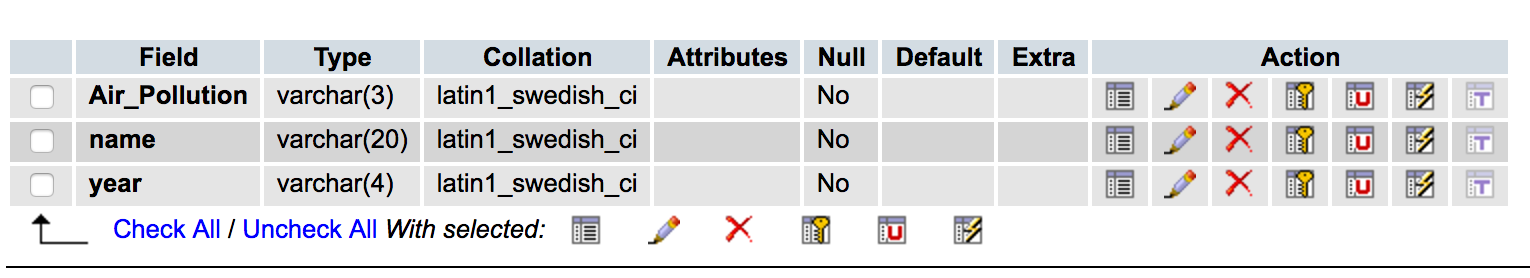
\includegraphics[width=\columnwidth]{air_poll_db.png}
\caption{The "air pollution" table's columns include "air pollution", "name", and "year" with "air pollution" 
containing all the values of the air pollution for each state and year, and "name" and "year" serving as keys.}
\label{fig:airPoll}
\end{figure}

\subsection{Design of the Interface}

\begin{figure}
\centering
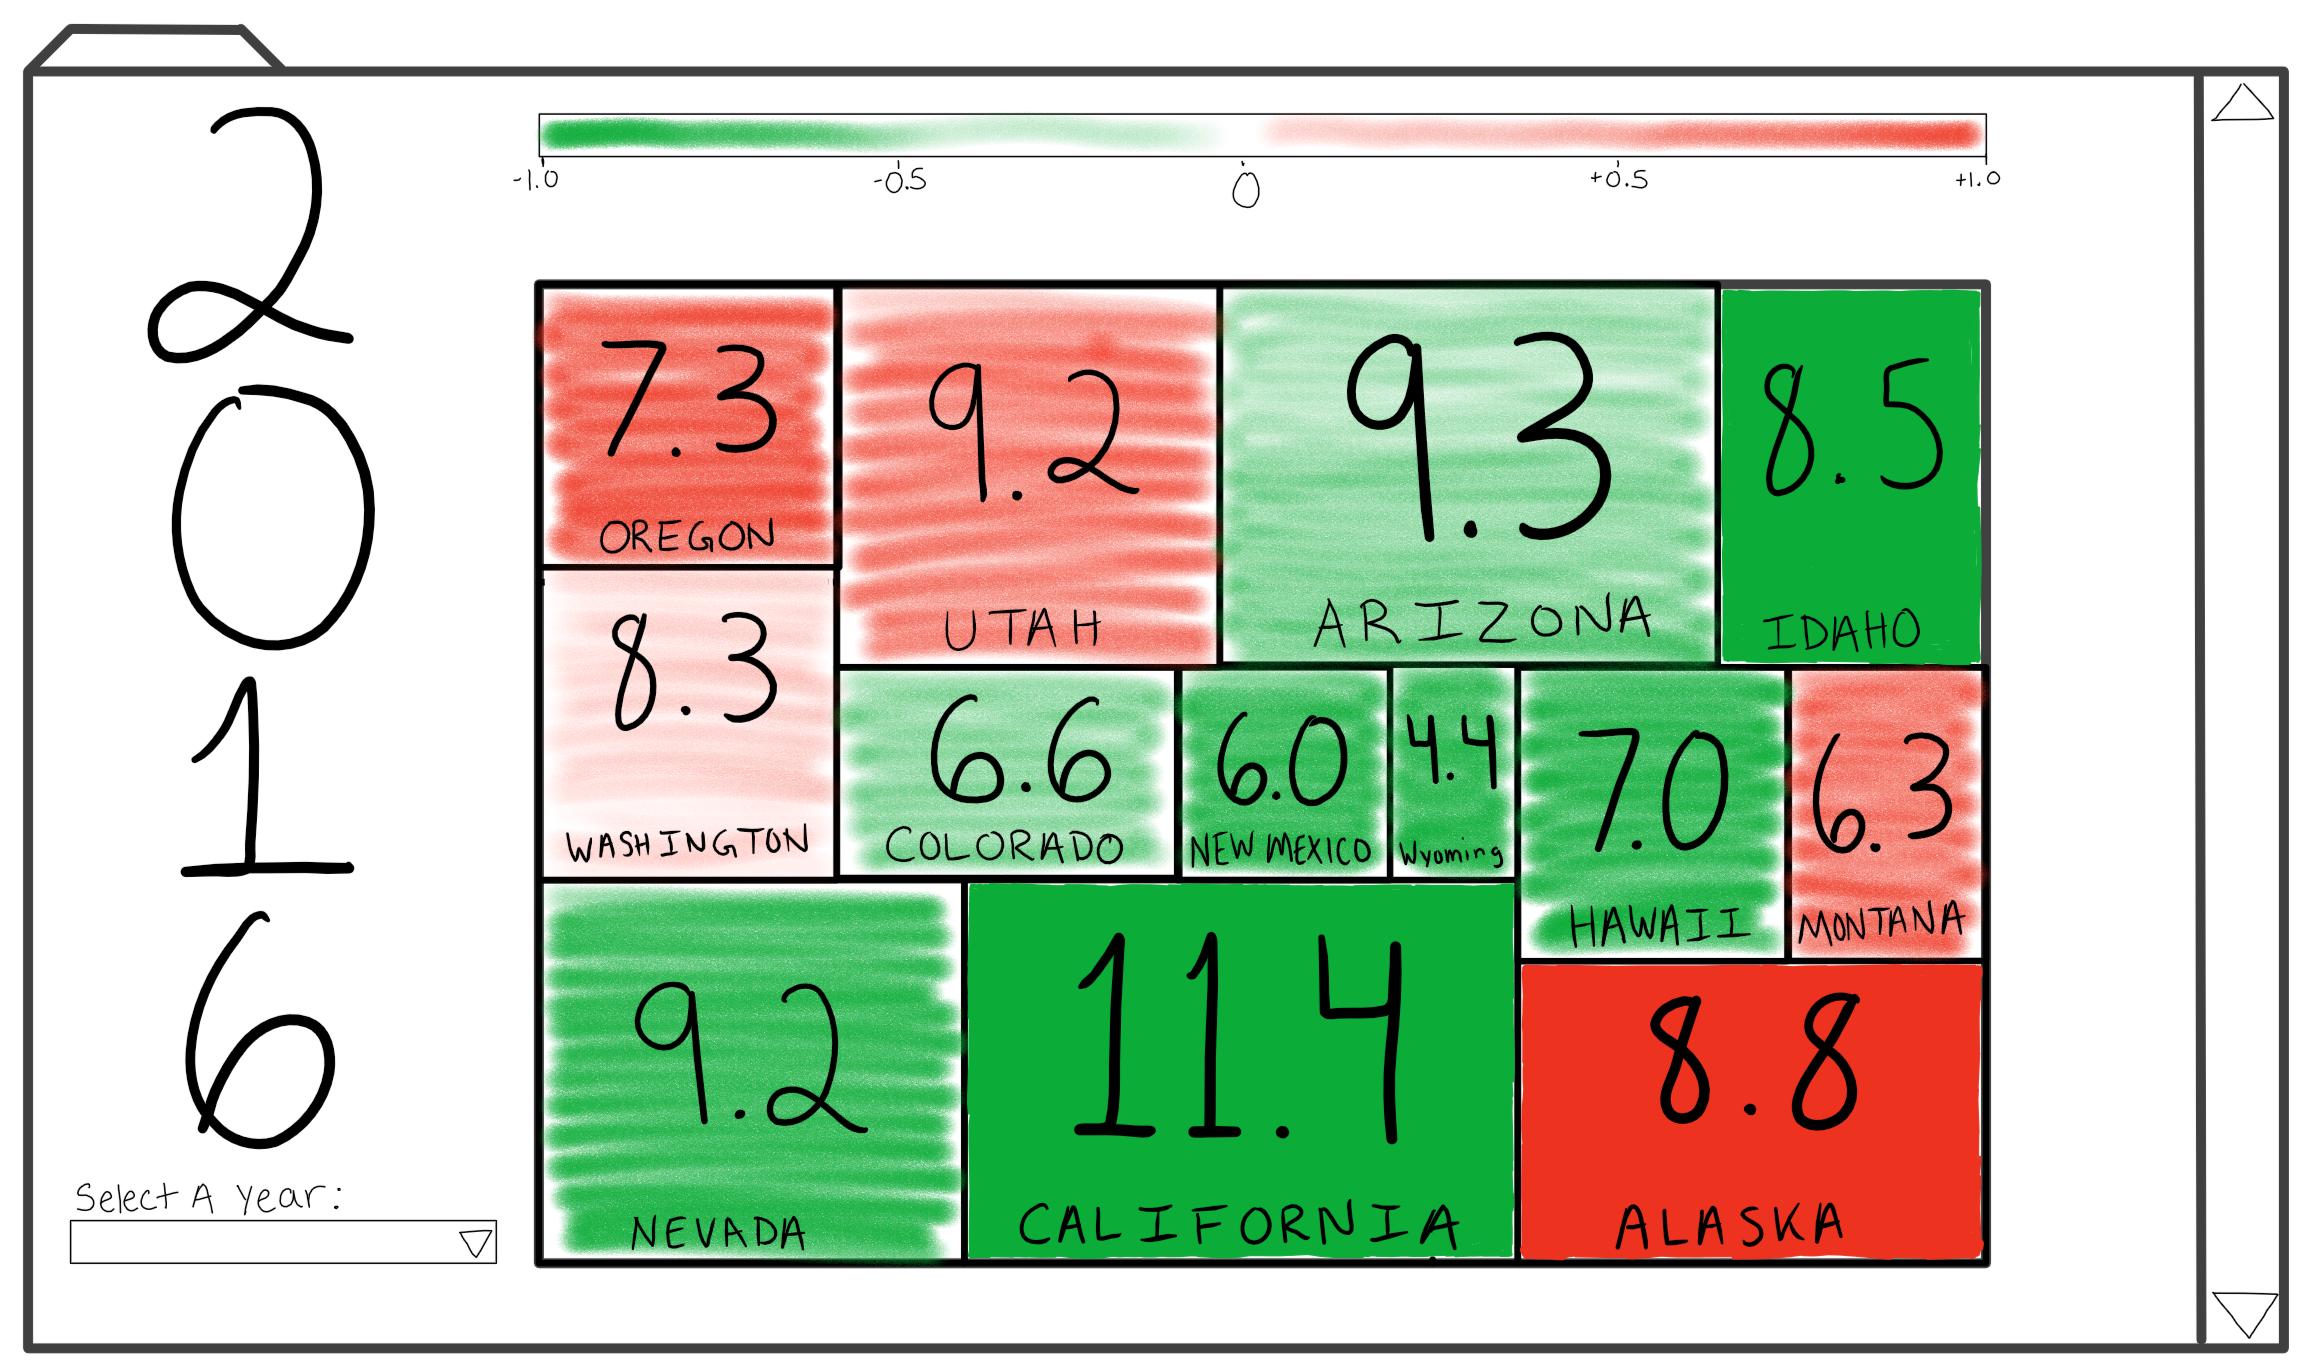
\includegraphics[width=\columnwidth]{HW1Design.PNG}
\caption{Our initial design for a visualization using a tree map describing the levels of air pollution in the western region by block size. See the text for more description.}
\label{fig:Design}
\end{figure}

We represent our data using an interactive tree map on a webpage. On the left hand side, users can select what year 
they want to view from 2007 to 2016, giving them the ability to see the changes in air pollution over the years. The 
size of the boxes on the tree map represent the magnitude of air pollution in a state in parts per million of harmful particulate matter. The larger the 
box, the higher the level of air pollution. The color of each box represents the change in air pollution levels from the previous 
year to the one selected. There will also be a scale above the treemap indicating what the range of the changes are for that year. 
A more negative number represents a higer decrease in harmful particulate levels - that is, a negative number means
that the state's air quality improved since the last measurement. On the other hand, a positive number represents an increase in harmful
particulate matter - and thus a decrease in air quality. The saturation of each box's color will serve as an indicator for the state's 
air quality. Our initial design for the visualization is represented in Figure \ref{fig:Design}.

\subsection{Enhancement Over Existing Models}

After reviewing the current models available, our model provides an enhancement by providing an easy-to-understand
metaphor for non-experts to view how their state's air pollution is changing over time. We achieve this through size
and color changing to represent whether the air pollution levels are rising or lowering over time. For example, a dark
orange block means that a state's air pollution level is rapidly increasing.

Previous models require an understanding of atmospheric sciences and are designed in mind for policy makers in the domain
of city planning[Zahran et al.]. While users with more experience in the domain of atmospheric sciences may use our
software, we hope to create a visualization that is accessible to users of all backgrounds.

\section{Implementation}

\subsection{Data Organization}
We created a relational database with 3 tables to store our data. The "state" table and "year" database are used to
index values stored within the "air pollution" database, as seen in the ER diagram in Figure \ref{fig:ERdiagram}.
We implemented the database on the ONID Database Server provided by Oregon State University. The contents
of the "state" diagram can be seen in Figure \ref{fig:stateDB} and the "air pollution" configuration can be found in 
Figure \ref{fig:airPoll}.

\subsection{Website}

\begin{figure}
   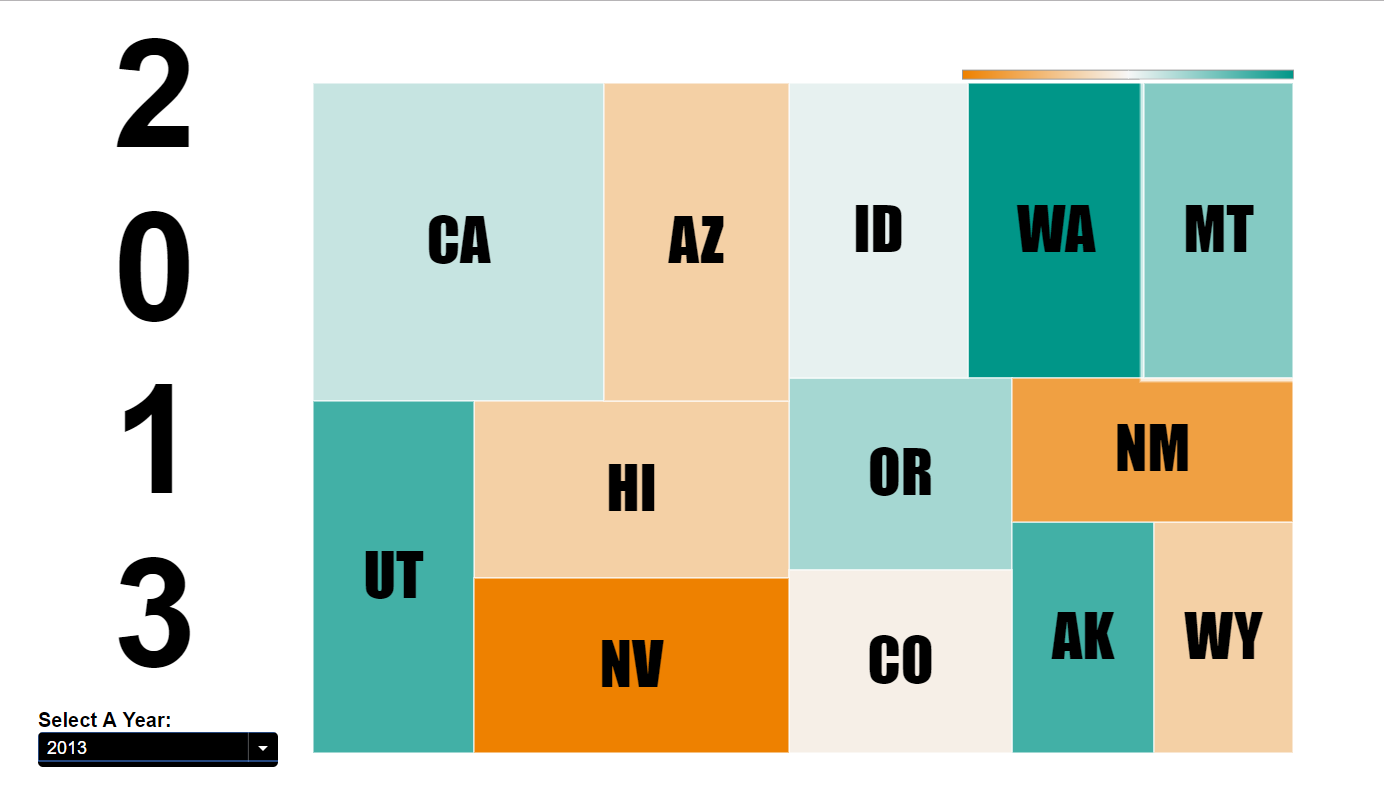
\includegraphics[width=\columnwidth]{2013_viz.png}
   \caption{A screenshot from our implemented website visualizing air pollution levels in the Western US. The user can select which year's data they
   would like to view using the dropdown menu. \label{fig:screenshot_all}}
\end{figure}

\begin{figure}
   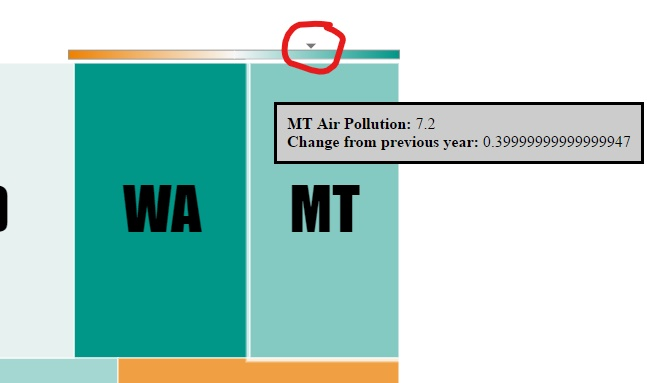
\includegraphics[width=\columnwidth]{screenshot_hover.jpg}
   \caption{A screenshot from our implemented website visualizinng air pollution levels in the Western US. The user can hover over a state's block
   to reveal a tooltip that contains information about a state's pollution levels for that year. Here, we see that Montana had a pollution level of
   7.2ppm of harmful particulate matter in the given year, which is a decrease of 0.399 ppm from the previous year. The red circle highlights the arrow
   that appears on the scale when hovering over the block that indicates where a state is in relation to others, to provide a means of comparison 
   with other states.\label{fig:screenshot_hover}}
\end{figure}


To implement our design, we decided to create a webpage that would display the data and provide ways for the user to
interact with the visualization. A screenshot of this website can be seen in Figure \ref{fig:screenshot_all}.
This website is live, and can be viewed and interacted with at the following link:
\url{http://infovizhw2.s3-website-us-west-2.amazonaws.com/}.

As mentioned before, we used Amazon Web Services (S3 bucket) to host our website and our database of information. This allowed us to
use the Google Charts library as a framework for our treemap. We leveraged the Charts API and Amazon's Lamdba service to build our treemap, querying our
database on page load and then feeding the resulting data into the JSON treemap object. Since we had ten years' worth of data to
visualise, we decided to create each year's treemap on an "as needed" basis - that is, we create the 2007 (default) treemap when the
page is initially loaded, then create each subsequent year's treemap as the user selects each year from the dropdown menu.
This allowed us to optimize the initial loading speed of the page - since it only has to render one treemap on load, instead of
ten, the page shows up much faster.

In addition, to provide some interactivity and clarity to the visualization, we give users the ability to hover over a block to 
gain more information about the state represented by that block (see Figure \ref{fig:screenshot_hover}). This tooltip gives the user the
exact measure of air pollution levels in parts per million of that state in the chosen year. It also provides the user information about
how much the magnitude of pollution changed from the previous year. In this way, the user has direct access to the data if they so desire it - 
giving them flexibility in how they interact with the visualization and increasing its utility.

\subsection{Issues Encountered and Resulting Design Choices}

As with any visualization project, there were some unexpected issues encountered in our implementation. 

First, we initially intended to host our website and database on the OSU servers, since that was the platform that we were
most familiar with. However, we found out during implementation that we could not leverage the Google Charts API if we did
this. As a result, we moved our development to Amazon Web Service's databases and servers, which had fewer restrictions on 
how APIs could be used. Though this changed where our visualization was hosted, it required only minimal modifications to 
our code and overall allowed us to create a better end product.

Second, as seen in our initial design (Figure \ref{fig:Design}), we planned to use red and green coloring for the treemap components, mapping
decreasing (better) air pollution levels to various saturations of green and increasing (worse) air pollution levels to reds. We believed
that this would intuitively make the "most sense" to the user, since green is "good" and red is "bad" in many visualizations. However, when
one of our group members spoke with the class's teaching assistant, he pointed out that red-green colorblindness is the most common form of
colorblindness. Thus, by choosing red and green, we made our visulaization virtaully useless to a small but significant subset of the population.
To address this, we changed our color scheme to orange and blue gradients, where blue is a decreasing (better) level of air pollution and orange
is an increasing (worse) level of pollution. As before, more saturated colors represent higher rates of change from year to year. This simple change
increased the usability of our visualization and furthered the ever-present goal of accessibility in public softwares.

Third, we encountered an issue in early devlopment where certain values larger than 10.0 would display incorrectly as 9.9. This was quickly
found to be a bug in the database settings - the database capped display of numbers at two digits. We were able to remedy this by changing 
a setting in the database options and explicitly stating in the code that we wanted more than two digits to display. 

Finally, when we finished the visualization and deployed it to a live site, we realized that there was a logical error in our code
that caused the first year of information (2007) to show incorrectly. This arose from how we structured our code: when we build a 
treemap and determine what colors the blocks should be, we use the data from the previous year's measurements to determine the saturation
and hue of each block's color. Since we do not have measurements from prior to 2007, we did not have a value to compare 2007's measurements
against. Due to the way we calculated the change, this missing value caused all the blocks in the 2007 treemap to appear dark orange - implying
every state's air pollution levels had increased drasically since the last year. Since this is likely incorrect, we decided to make 2007's blocks
all grey in color, indicating no measured change from the previous year. Though this does make the 2007 treemap lack one dimension of the information
we are visualizing, we thought this would be the best way to avoid misrepresenting data that we didn't have, leading to a more accurate
visualization overall.

\section{Results}

\subsection{Insights}

Visualizing the air pollution data in this way reveals some interesting insights.

First of all, we found that there was no overall, unifying trend to the level of air pollution in the Western US
over the past ten years. This was surprising, because we expected to see something - either a general increase in air quality
(which would suggest that climate change initiatives were effective) or a general decrease in air quality (which
would suggest that climate change was damaging air quality faster than we could combat it). Instead, we didn't see any clear 
trend to the direction of air quality fluctuations. There were periods of constantly increasing air quality for the majority 
of states (e.g., 2010-2011), but these periods were followed by a sharp decrease in air quality (e.g. 2012). See Figures \ref{fig:2011_viz}
and \ref{fig:2012_viz} for a visual comparison of these phenomena.

\begin{figure}
   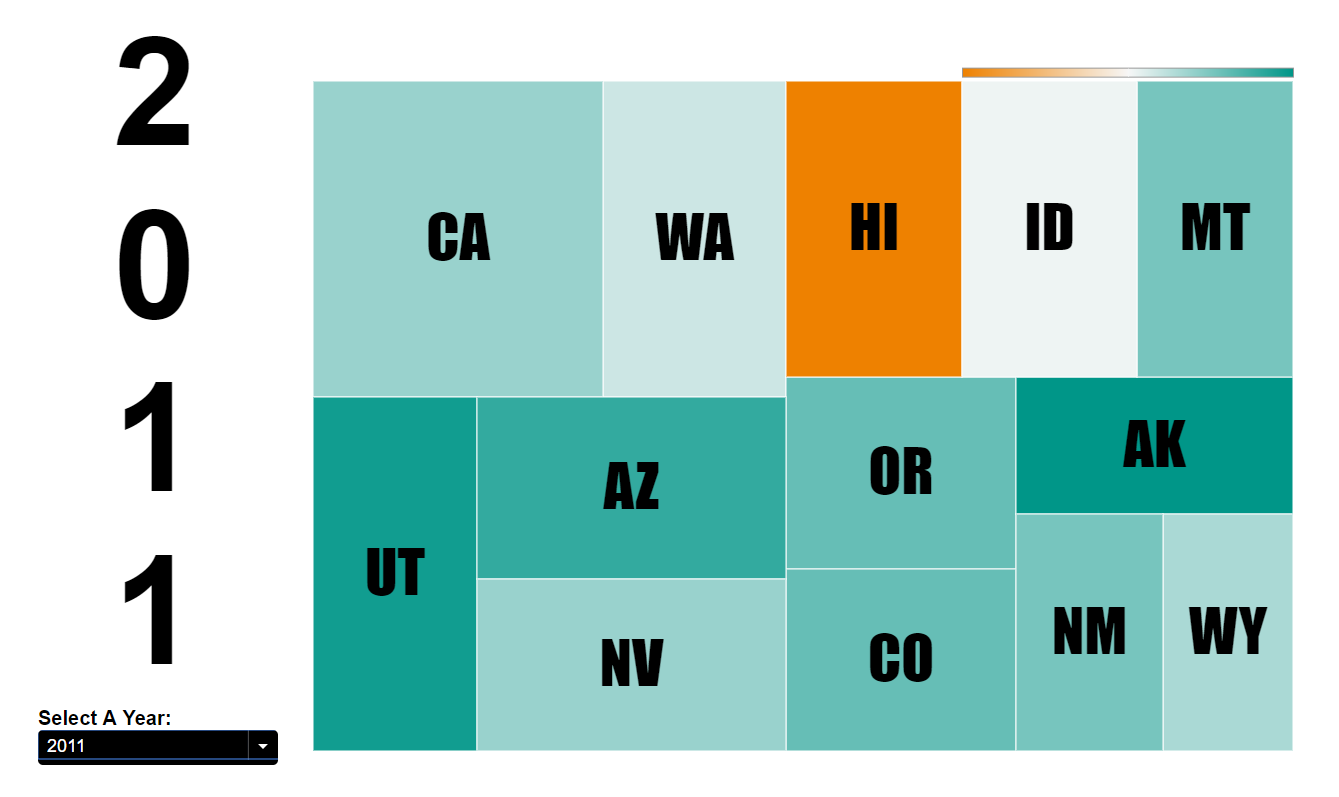
\includegraphics[width=\columnwidth]{2011_viz.png}
   \caption{A screenshot of our visualization for the year 2011. The majority of the states showed moderate to large increases
   in air quality from the year before, as evidenced by most of the blocks being a shade of blue rather than orange. \label{fig:2011_viz}}
\end{figure}

\begin{figure}
   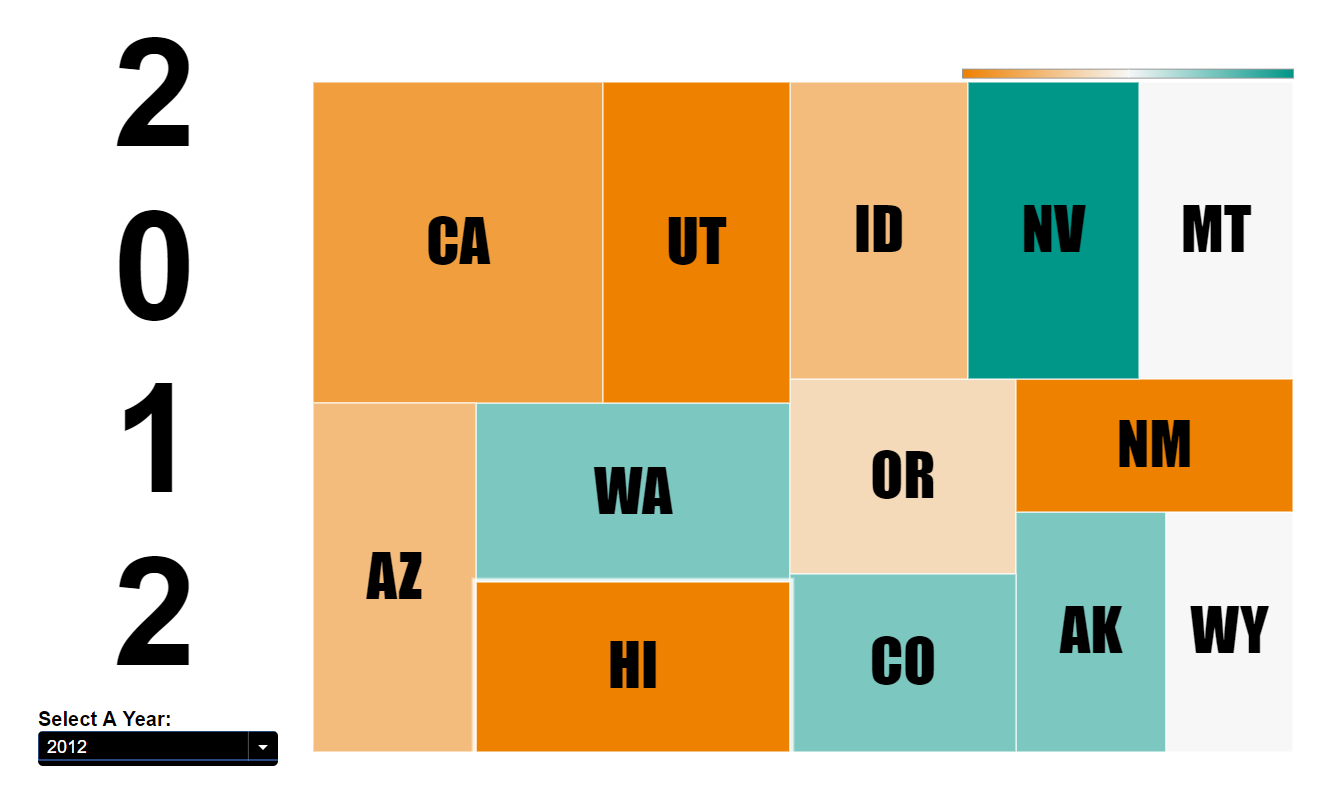
\includegraphics[width=\columnwidth]{2012_viz.png}
   \caption{A screenshot of our visualization for the year 2012, directly after the previous figure. Here, the majority of states
   showed decreases in air quality, as evidenced by most blocks being a shade of orange.\label{fig:2012_viz}}
\end{figure}

When looking at individual states, however, we did see trends. For example, California consistently had the largest amount of air
pollution over the time span of the visualization, regardless of whether the levels increased or decreased from the previous year.
Interestingly, in 2015 and 2016, Idaho was almost tied with California for the highest amonut of air pollution - but at the end
of the visualization time span, California's air quality was getting better, while Idaho's was getting worse.

Hawaii and Wyoming were roughly tied for the lowest consistent amount of pollution from the beginning of the time span until about 2011, when Hawaii
experienced a sharp decline in air quality and Wyoming suddenly experienced better air. (An example of this can be seen in \ref{fig:2011_viz}).
Since that time, until the end of the visualization time span, Wyoming consistenly had the lowest amount of air pollution. 

Looking at this model through the eyes of someone who might want to move to one of these states, some regions are certainly better choices than 
others. For instance, a person with asthma or breathing difficulties would probably not want to move to Alaska in the near future - though
the state was never the worst offender in terms of air quality levels, Alaska's pollution levels showed a sharp increase in the later few
years of the visualization - indicating that Alaska might soon become a low air quality state. On the other hand, this person might consider
a move to Montana - the rural state had a consistently low level of air pollution (though never the actual least), and was almost always
colored blue, which indicates a steady increase in air quality.

\subsection{Data Set}

As mentioned in the Methods section, we used ten years' worth of air pollution data from the United Health Foundation's
website on the topic. See that section for a more detailed description of how we obtained the data. 
This gave us a set consisting of 110 data points (11 states x 10 years) that we leveraged to build our visualizaton. 

\subsection{Dimensions Used}

Our visualization models two dimensions of the data. First, it maps the magnitude of a state's pollution levels to 
the spatial domain using the size of the block in the treemap. A larger block corresponds to higher levels of pollution, 
while a smaller block means lower pollution levels. In a way, the spatial dimensions of each block can be though of as 
"how big" the state's contribution is to the overall level of air pollution in the Western US.

Second, we represent the temporal dimension of the data (over a span of 10 years) through the relative, changing colors of each block
in the treemap. When viewing a given year's treemap, the color of the blocks indicates the change in air pollution levels 
from the previous year. This gives a sense of time to the data and firmly grounds our model in the temporal domain. Without
this dimension, it would be much harder to find interesting trends over time - we would have no mechanism to directly compare 
across years.

\subsection{Performance}

Our visualization performed well in its intended task. It gave an efficient and effective overview of air quality in this 
region of the country and allowed not only the identification of certain "problem" states that had persistently bad
air quality, but also the states that would be more likely to maintain their good air quality in the future.

However, as with any visualization, there were a few drawbacks to representing data in this fashion. For instance, as discussed
in the Insights section, we could not discern any overall trend to the data. One explanation for this is that there really was
not any trend - that the fluctuations did not follow any pattern. Another explanation is that there was a trend that we were not
able to figure out with this method of visualization. This is a possible idea for future work in this area. 

\subsection{Supplementary Materials}

We used GitHub to organize our materials and code for the paper and the website. 

Paper repository: \url{https://github.com/horvathaa/cs458/}

Visualization repository: \url{https://github.com/kbajno/cs458-assign2/}

The visualization website itself can be viewed and interacted with at 
\url{http://infovizhw2.s3-website-us-west-2.amazonaws.com/}.


\subsection{Domain Expert Review}

Since one of our group members intends to live in the Western US when she gradutes and 
is interested in air quality indices for the geographic regions, we had her act as the 
domain expert for reviewing a visualization. She has taken two environmental science 
classes that covered the causes and effect of air pollution in detail, so she has
enough background experience to count as one with domain knowledge in this case.

Overall, the expert was positive towards our visualization. She mentioned that she was
able to get a good overall feel for the data at a high level, and liked that the user
could click or hover on each state to gain deeper insights into the data. She was able
to use our visualization to track Oregon across the ten years and was pleased to find
that the state never showed any huge increases in air pollution levels (Oregon tended
to stay roughly the same across the time span). 

One criticism she had, however, was that it was somewhat difficult to see how certain 
states compared across the years. With the way that the Google Charts API builds a 
treemap, the size of the blocks determines the order in which they appear in the map. 
This can lead to confusion when certain states experience significant changes in the 
magnitude of their air pollution - the state's block might move from the left side of
the map one year to the right side in the next year. In this way, she suggested that
we consider freezing the states in place relative to each other to make comparisons
across time easier at a glance.


\section{Conclusion and Future Work}

Overall, our visualization proved successful for showcasing differences
in air pollution levels over time in the western United States region.
As referenced in our Related Works section, this visualization improved
over previous works by being easily understood by a crowd with minimal to no experience in 
air pollution research
and allowed for comparisons between regions as opposed to purely within
a single region. The implementation proved to be relatively
easy to create and run on different computers. As a proof of concept, this endeavor proved to be
successful.

When reviewing the data, we found some interesting findings. As mentioned in Results, there was no unifying
trend in air pollution in the western United States over the past 10 years. With the general consensus in the media
stating that air pollution is increasing at a concerning rate, it might relieve people interested in
moving to the western United States that, while air pollution might be bad in individual states, the overall region
is not experiencing a dangerous increase in air pollution. However, as mentioned in the Results section, a trend might
appear if we were to support more visualizations of the data we have found for the western region. While we believe this is unlikely,
supporting multiple views might aid other research questions or lead to more interactability with the application.

We also found that individual states experienced some drastic changes in air pollution levels. California maintained a high amount of air pollution
throughout the 10 years worth of data that we had, but Idaho, in the years 2015 and 2016, began catching up to California in terms of air pollution.
What this might suggest is that either Idaho's endeavors in combating air pollution failed and it's increase in population began to catch up
to it, or that California began better combating it's consistently high air pollution levels.  

At this point, a supporting visualization
that allows for cross-comparison between two chosen states could shed light onto this interesting finding. Or providing more metadata about
how the air pollution levels were distributed throughout the state (i.e. perhaps northern Idaho has clean air, but southern Idaho is skewing the
results with a high amount of pollution). Another option to support comparing between states is to freezing states in place on the map, as
noted by our domain expert. While this wouldn't allow for the level of granularity previously described, it would still make for a better
user experience by supporting comparison between states and also easing a new user into using the application, as the obvious
interpretation of our visualization is that the states would be ordered depending upon their geographic location as opposed to their distribution
being based solely upon size.

In the future, we would like to enhance our visualization based upon both previous work and the insights we gained during
the implementation and reviewing process. Previous work, such as [Elbir et al.] use the data they've received to predict future
levels of air pollution. Enhancing our model to predict future air pollution levels statewide would further our goal of informing
the population about how their state is doing in comparison to other states and against itself. Furthermore, it would allow
users from other states to see if they should move away to a cleaner state if they're concerned about air pollution. 

\section{Acknowledgements}

We would like to thank Oregon State University, Eugene Zhang, and the United World Health Foundation for
making this research possible.

\section{References}
[1] 

\end{document}

